\documentclass{beamer}
%\documentclass[handout]{beamer}

\mode<presentation>
{
  \usetheme{Montpellier}

  %\setbeamercovered{transparent}
  % or whatever (possibly just delete it)
}

\usepackage{xmpmulti} % package that defines \multiinclude

\usepackage[english]{babel}

\usepackage[latin1]{inputenc}

\usepackage{times}
\usepackage[T1]{fontenc}
% Or whatever. Note that the encoding and the font should match. If T1
% does not look nice, try deleting the line with the fontenc.

\newcommand{\newmcommand}[2]{\newcommand{#1}{{\ifmmode {#2}\else\mbox{${#2}$}\fi}}}
\newcommand{\renewmcommand}[2]{\renewcommand{#1}{{\ifmmode {#2}\else\mbox{${#2}$}\fi}}}
\newcommand{\newmcommandi}[2]{\newcommand{#1}[1]{{\ifmmode {#2}\else\mbox{${#2}$}\fi}}}
\newcommand{\newmcommandii}[2]{\newcommand{#1}[2]{{\ifmmode {#2}\else\mbox{${#2}$}\fi}}}
\newcommand{\newmcommandiii}[2]{\newcommand{#1}[3]{{\ifmmode {#2}\else\mbox{${#2}$}\fi}}}

\newcommand{\algfnt}{\bf}

\newmcommand{\ouralg}{{\mbox{\algfnt Hedge}({\eta})}}

\newmcommand{\iter}{T}

\newfont{\cmmib}{cmmib10}
\newcommand{\boldell}{{\mbox{\cmmib \symbol{'140}}}}


\newmcommandi{\costvec}{{\boldell}^{#1}}
\newmcommandii{\cost}{{\ell}^{#1}_{#2}}

\newmcommandi{\rd}{\tilde{#1}}

\newmcommandi{\distvec}{{\bf p}^{#1}}
\newmcommandi{\rddistvec}{\rd{\bf p}^{#1}}
\newmcommandii{\dist}{{p}^{#1}_{#2}}
\newmcommandii{\rddist}{\rd{p}^{#1}_{#2}}

\newmcommandi{\bdistvec}{{\bf q}^{#1}}
\newmcommandii{\bdist}{{q}^{#1}_{#2}}

\newmcommandi{\wtvec}{{\bf w}^{#1}}
\newmcommandi{\rdwtvec}{\rd{\bf w}^{#1}}
\newmcommandii{\wt}{{w}^{#1}_{#2}}
\newmcommandii{\rdwt}{\rd{w}^{#1}_{#2}}


\newcommand{\Nweight}[2]{V_{#1}^{#2}}	%the normalized weight
\newcommand{\dweight}[2]{w^{#2}(#1)} % initial density measure
\newcommand{\TEloss}[1]{L_{#1}}	%total loss of expert i
\newcommand{\BEloss}{L_{\min}}	%total loss of the best expert
\newcommand{\TAloss}{L_A}	%total loss of algorithm
\newcommand{\weight}[2]{W_{#1}^{#2}} % weight assigned to expert
\newcommand{\btheta}{\hat{\theta}}

\newcommand{\R}[1]{{\color{red}{#1}}}
\newcommand{\B}[1]{{\color{blue}{#1}}}
\newcommand{\RM}[1]{{\color{red}{$#1$}}}


%BANDITS
\newcommand{\Aplay}{{\bf Hedge}}
\newcommand{\Aest}{{\bf Exp3}}
\newcommand{\Aesthp}{{\bf Exp3.P}}
\newcommand{\Aestg}{{\bf Exp3.P.1}}
\newcommand{\Aests}{{\bf Exp3.S}}
\newcommand{\Aessg}{{\bf Exp3.S.1}}
\newcommand{\Astrat}{{\bf Exp4}}
\newcommand{\Abound}{{\bf Exp3.1}}
\newcommand{\Gbest}{G_{\rm max}}

\newcommand{\defeq}{\stackrel{\rm def}{=}}
\newcommand{\compl}{\mbox{\sc h}}
\newcommand{\theset}[2]{\{ {#1} \,:\, {#2} \}}

\newmcommandii{\stratv}{\mbox{\boldmath $\xi$}^{#1}({#2})}

%Games paper
\newmcommand{\M}{\bf M}
\newmcommand{\dM}{\M'}
\newmcommand{\Row}{\bf R}
\newmcommand{\dRow}{\R'}
\newmcommand{\C}{\bf C}
\newmcommand{\dC}{\C'}
\newmcommand{\D}{D}
\renewmcommand{\P}{\bf P}
\newmcommand{\Q}{\bf Q}
\newmcommand{\Dt}{\D_t}
\newmcommand{\Pt}{\P_t}
\newmcommand{\Qt}{\Q_t}
\newmcommand{\Pstar}{\P^*}	% the min/max optimal mixed strategy
\newmcommand{\Pref}{\tilde{\P}}	% a reference mixed strategy (not
				% necessarily min/max)
\newmcommand{\Qstar}{\Q^*}
\newmcommand{\Pa}{\overline{\P}}
\newmcommand{\Qa}{\overline{\Q}}
\newmcommand{\Qh}{\hat{\Q}}
\newmcommandi{\trans}{{#1}^{\rm T}}
\newmcommand{\mhx}{\M(h,x)}
\newmcommand{\mxh}{\dM(x,h)}
\newmcommand{\mpq}{\M(\P,\Q)}
\newmcommand{\mpsq}{\M(\Pstar,\Q)}
\newmcommand{\mpsqt}{\M(\Pstar,\Qt)}
\newmcommand{\mptqt}{\M(\Pt,\Qt)}
\newmcommand{\mptt}{\M(\Pt,t)}
\newmcommand{\mptq}{\M(\Pt,\Q)}
\newmcommand{\mpqt}{\M(\P,\Qt)}
\newcommand{\minp}{\min_{\P}}
\newcommand{\maxq}{\max_{\Q}}
\newcommand{\RE}[2]{{\rm RE}\left( {#1} \; \parallel \; {#2} \right) }

\newmcommand{\sumt}{\sum_{t=1}^T}
\newmcommand{\sumin}{\sum_{i=1}^n}
\newmcommand{\delt}{\Delta_{T,n}}
\newcommand{\nextline}{\vspace{0.2cm}\\}   % a little space for equation arrays

\newcommand{\lwalg}{\mbox{\rm MW}}
\newcommand{\lwalgvar}{\mbox{\rm vMW}}

%%
\newcommand{\E}{\mbox{\rm\bf E}}
\newcommand{\p}[2]{p_{#1}(#2)}
\newcommand{\q}[2]{q_{#1}(#2)}
\newcommand{\x}[2]{x_{#1}({#2})}
\newmcommand{\bx}{\mbox{\boldmath$x$}}
\newmcommandi{\xv}{\bx({#1})}
\newmcommand{\xvt}{\xv{t}}
%\newcommand{\w}[2]{w_{#1}({#2})} replaced by \wt, but remember to switch order of parameters i and t
\renewcommand{\i}[1]{i_{#1}}
\newcommand{\hx}[2]{\hat{x}_{#1}(#2)}
\newcommand{\hxit}{\hx{\i{t}}{t}}
\newcommand{\pit}{\p{\i{t}}{t}}
\newcommand{\xit}{\x{\i{t}}{t}}
\newcommand{\expb}[1]{\exp\left(#1\right)}

\newcommand{\vp}{{\mathbf p}}
\newcommand{\vu}{{\mathbf u}}
\newcommand{\vv}{{\mathbf v}}
\newcommand{\vx}{{\mathbf x}}
\newcommand{\vy}{{\mathbf y}}

\newcommand{\HedgeLoss}{L_{\mbox{\footnotesize Hedge}}}

\newcommand{\W}{\vec{W}}
\newcommand{\V}{\vec{V}}
\newcommand{\X}{\vec{X}}
\newcommand{\vb}{\vec{b}}
%\newcommand{\loss}{\vec{\ell}}
\newcommand{\loss}{L}
%\newcommand{\elloss}[2]{\ell_{#1}^{#2}} %loss of expert i at time t
\newcommand{\elloss}[2]{\ell_{#2}\left( #1 \right)} %loss of expert i at time t
\newcommand{\w}[1]{\makebox[12pt]{{#1}}}
\newcommand{\Rps}{\mbox{\tt R}}
\newcommand{\rPs}{\mbox{\tt P}}
\newcommand{\rpS}{\mbox{\tt S}}
\newcommand{\rpstie}{\w{$\frac{1}{2}$}}
\newcommand{\rpswin}{\w{$0$}}
\newcommand{\rpsloss}{\w{$1$}}

\newmcommand{\decspace}{\Delta}
\newmcommand{\decsym}{\delta}
\newmcommandi{\dec}{\decsym^{#1}}
\newmcommand{\decdistsym}{\cal D}
\newmcommandi{\decdist}{{\decdistsym}^{#1}}

\newmcommand{\simpdistspace}{{\bf \cal S}}
\newmcommand{\domset}{{\rm dom}(\decdistsym)}

\newmcommand{\expdistsym}{{\cal E}}
\newmcommandii{\expdist}{{\expdistsym}^{#1}_{#2}}
\newmcommand{\expdecsym}{{\varepsilon}}
\newmcommandii{\expdec}{\expdecsym^{#1}_{#2}}

\newmcommand{\outspace}{\Omega}
\newmcommand{\outsym}{\omega}
\newmcommandi{\out}{\outsym^{#1}}

%\newmcommandii{\Dkl}{D_{\mbox{kl}}\paren{#1||#2}}
\newmcommandii{\Dkl}{{\rm {KL}}\paren{{#1}\;||\;{#2}}}

\newmcommandi{\sumwts}{\sum_{i=1}^N \wt{#1}{i}}

\newmcommand{\lossalg}{L_A}
\newmcommand{\lossouralg}{{L_{\mbox{\scriptsize\algfnt Hedge}(\eta)}}}
\newmcommand{\lossS}{{L_{\mbox{\scriptsize\algfnt S}}}}
\newmcommandi{\lossi}{L_{#1}}
\newmcommandii{\lossit}{L_{#1}^{#2}}

\newmcommandi{\upbnd}{\tilde{#1}}

\newcommand{\angles}[1]{{\left\langle {#1} \right\rangle}}
\newcommand{\paren}[1]{{\left( {#1} \right)}}
\newcommand{\brac}[1]{{\left[ {#1} \right]}}
\newcommand{\braces}[1]{{\left\{ {#1} \right\}}}

\newcommand{\abs}[1]{{\left| {#1} \right|}}
\newcommand{\ceiling}[1]{{\left\lceil {#1} \right\rceil}}

\newfont{\msym}{msbm10}
\newcommand{\real}{\mbox{\msym R}}

\newmcommand{\updatefcn}{U_\eta}

%% \newtheorem{theorem}{Theorem}	
%% \newtheorem{lemma}[theorem]{Lemma}
%% \newtheorem{corollary}[theorem]{Corollary}
%% \newtheorem{definition}{Definition}

%\newcommand{\proof}{\noindent{\bf Proof:} }
%\newcommand{\example}[1]{{\em Example #1.} }
%\newcommand{\qed}{\rule{0.7em}{0.7em}}

\newcommand{\WeakAlg}{\mbox{\algfnt WeakLearn}}
\newcommand{\Boost}{\mbox{\algfnt AdaBoost}}
\newcommand{\EX}{\mbox{\bf EX}}
\newmcommand{\hf}{h_{{f}}}
\newmcommand{\rdhf}{\rd{h}_{{f}}}
\newmcommand{\hfT}{h^T_{{f}}}
\newmcommand{\ranh}{{b}}

\newmcommand{\conclass}{{\cal C}}

\newmcommand{\badvec}{{\bf b}}
\newmcommandi{\bad}{{b}_{#1}}

%%%%%%%% New commands defined for the game-playing paper

\newmcommand{\hedge}{\algfnt Hedge}
\newmcommand{\play}{\algfnt Play}
\newmcommandi{\Glossvec}{{\bg y}^{#1}}
\newmcommandii{\Gloss}{{y}^{#1}_{#2}}
%\newmcommandi{\action}{{I}_{#1}}
\newmcommandi{\Gdistvec}{{\bf \tilde{p}}^{#1}}
\newmcommandii{\Gdist}{{\teilde{p}}^{#1}_{#2}}

%%%%%%%%%%%%%%%%%%%%%%%%%%%%%%%%%%%%%%%%%%%%%%%%%%%%%
\newmcommand{\Idistvec}{{D}}
\newmcommandi{\Idist}{\Idistvec({#1})}
\newmcommand{\Idistt}{\Idistvec_t}

\newmcommand{\Xdist}{{\cal P}}
\newmcommand{\emp}{\hat{\epsilon}}

\newmcommand{\classpc}{Y}
\newmcommand{\numclass}{k}
\newmcommandii{\prob}{\mbox{\rm Pr}_{#1}\left[{#2}\right]}
\newmcommandii{\exval}{\mbox{\rm E}_{#1}\left[{#2}\right]}

%\usepackage{amsmath}
\DeclareMathOperator*{\argmax}{argmax} % thin space, limits underneath in displays
\DeclareMathOperator*{\argmin}{argmin} 

\newcommand{\RR}{\mathbb{R}}
\newcommand{\regret}{\mbox{Regret}}

%%% Conditional probabilities
\newmcommandii{\condp}{p\left( #1 \left| #2 \right. \right)}

\newmcommand{\lab}{y}
\newmcommand{\ploss}{\mbox{ploss}}
\newmcommandii{\avploss}{\ploss_{#1}({#2})}
\newcommand{\sfrac}[2]{\mbox{$\frac{#1}{#2}$}}

\newcommand{\mboosta}{\mbox{\algfnt AdaBoost.M1}}
\newcommand{\mboostb}{\mbox{\algfnt AdaBoost.M2}}
\newcommand{\mboostr}{\mbox{\algfnt AdaBoost.R}}

%\newmcommand{\slos}{\mbox{ploss}}
%\newmcommandiii{\sloss}{\slos_{#1}({#2},{#3})}
%\newmcommandiii{\avsloss}{\slos_{{#1},{#2}}({#3})}

\newmcommandii{\vwt}{{W}^{#1}_{#2}}

\newcommand{\figline}{\rule{\textwidth}{1pt}}

%\newmcommandi{\1}{{\bf 1}({#1})}
\newmcommandi{\1}{[\![{#1}]\!]}

\newmcommand{\confcn}{\kappa}
\newmcommandi{\erint}{\abs{\int_{y_i}^{h_t(x_i)} {#1} dy}}
%\newmcommandi{\erint}{\int_{\min\{y_i,h_t(x_i)\}}^{\max\{y_i,h_t(x_i)\}}{#1}dy}


\title[Introduction] % (optional, use only with long paper titles)
{Introduction to Online Learning Algorithms}

\author[Freund] % (optional, use only with lots of authors)
{Yoav Freund}
% - Give the names in the same order as the appear in the paper.
% - Use the \inst{?} command only if the authors have different
%   affiliation.

\institute[Universities of Somewhere and Elsewhere] % (optional, but mostly needed)

\subject{Machine Learning}
% This is only inserted into the PDF information catalog. Can be left
% out. 

% If you have a file called "university-logo-filename.xxx", where xxx
% is a graphic format that can be processed by latex or pdflatex,
% resp., then you can add a logo as follows:

% \pgfdeclareimage[height=0.5cm]{university-logo}{university-logo-filename}
% \logo{\pgfuseimage{university-logo}}



% Delete this, if you do not want the table of contents to pop up at
% the beginning of each subsection:
%% \AtBeginSubsection[]
%% {
%%   \begin{frame}<beamer>
%%     \frametitle{Outline}
%%     \tableofcontents[currentsection,currentsubsection]
%%   \end{frame}
%% }


% If you wish to uncover everything in a step-wise fashion, uncomment
% the following command: 

\beamerdefaultoverlayspecification{<+->}

% \newcommand{\W}{\vec{W}}
% \newcommand{\V}{\vec{V}}
% \newcommand{\X}{\vec{X}}
% \newcommand{\loss}{\vec{\ell}}
% \newcommand{\HedgeLoss}{L_{\mbox{\footnotesize Hedge}}}

\begin{document}

\begin{frame}
  \titlepage
\end{frame}

\begin{frame}
  \frametitle{Outline}
  \tableofcontents
  % You might wish to add the option [pausesections]
\end{frame}

%\iffalse %%%%%%%%%%%%%%%%%%%%%%%%%%%%%%%%%%%%%%%%%%%%%%%%%%%%%%%%%%%%%%%%%%
\section{Halving Algorithm}

\begin{frame} 
\frametitle{Example trace for Halving Algorithm} 

%\newcommand{\uncovered}[1]{\onslide<{#1}->\color<{#1}>{red}}

\begin{columns} 
\column[t]{3cm}
\onslide<1->\color<1>{red} 
~ \\ expert1\\ expert2\\ expert3\\ expert4 \\ expert5\\ expert6\\ expert7\\ expert8 \\ ~\\
\onslide<{2}->\color<2>{red} alg.\\
\onslide<3->\color<3>{red} outcome 
%\uncovered{3} outcome 

\column[t]{1cm}
\onslide<4->\color<4>{red} $t=1$   \\ 1 \\ 1 \\ 0  \\ 1 \\ 1 \\ 0 \\ 1  \\ 1 \\ ~ \\
\onslide<5->\color<5>{red} 1 \\
\onslide<6->\color<6>{red} 1 \\
		   			   
\column[t]{1cm}	   		   
\onslide<7->\color<7>{red} $t=2$   \\ 1 \\ 0 \\ -  \\ 0 \\ 0 \\ - \\ 1  \\ 1 \\ ~ \\
\onslide<8->\color<8>{red} 0 \\
\onslide<9->\color<9>{red} 1 \\

\column[t]{1cm}
\onslide<10->\color<10>{red} $t=3$ \\ 1 \\ - \\ -  \\ - \\ - \\ - \\ 1  \\ 1 \\ ~ \\
\onslide<11->\color<11>{red} 1 \\
\onslide<12->\color<12>{red} 1 \\
		    			     
\column[t]{1cm}	    		     
\onslide<13->\color<13>{red} $t=4$ \\ 1 \\ - \\ -  \\ - \\ - \\ - \\ 1  \\ 0 \\ ~ \\
\onslide<14->\color<14>{red} 1 \\
\onslide<15->\color<15>{red} 0 \\
		    			     
\column[t]{1cm}	    		     
\onslide<16->\color<16>{red} $t=5$ \\ - \\ - \\ -  \\ - \\ - \\ - \\ 0  \\ - \\ ~ \\
\onslide<17->\color<17>{red} 0 \\
\onslide<18->\color<18>{red} 0 \\

\end{columns} 
\end{frame} 

\begin{frame}
\frametitle{Mistake bound for Halving algorithm}
\begin{itemize}
\item 
Each time algorithm makes a mistakes, the pool of perfect experts is halved (at least).
\item
We assume that at least one expert is perfect.
\item
Number of mistakes is at most $\log_2 N$.
\end{itemize}
\end{frame}


\begin{frame}
\frametitle{Characteristics of individual sequence analysis}
\begin{itemize}
\item
No stochastic assumptions.
\item
  Proof is based on combining a lower and upper bounds on a \R{Potential}
\item Here, \R{Potential} = number of experts in pool.
\end{itemize}
\end{frame}

\begin{frame}
\frametitle{Optimality of Halving algorithm}
\begin{itemize}
\item Adversary chooses expert predictions and outcomes so as to
  maximize the number of mistakes.
\item
The best strategy for the adversary: split a pool with \R{$m$} experts
into \\
\R{$\lfloor m/2 \rfloor$} predicting 0 \\
\R{$\lceil m/2 \rceil$} predicting $1$\\
Make the actual output $0$.
\item The halving algorithm can be forced to $k^*$ mistakes. $k^* \leq
  \log N$.
\item \R{$k^ :$} $m_0=N$, $m_{i+1} = \lfloor m_i \rfloor$, $m_{k^*} = 1$.
\item If $N=2^k$ then $k^*=k$, otherwise $k^* < \log N$
\item $k^*$ is  the \B{Min-Max number of mistakes}: algorithm never
  makes more than $k^*$ mistakes, adversary can force $k^*$ mistakes.
\end{itemize}
\end{frame}

\section{Hedge Algorithm}

\begin{frame}
\frametitle{The hedging problem}

What should we do if none of the experts is perfect, and we have no
a-priori knowledge how good the best expert is?
\begin{itemize}
\item $N$ possible actions 

\item At each time step $t$:
\begin{itemize}
\item Algorithm chooses a distribution $\vec{P}^t$ over actions.
\item Losses $0 \leq \ell_i^t \leq 1$ of all actions $i=1,\ldots,N$ are revealed.
\item Algorithm suffers {\bf expected} loss.
\end{itemize}
\item {{\bf Goal:} minimize total expected loss}
\item {Here we have stochasticity - but only in {\bf algorithm}, not in {\bf outcome}}
\item {Fits nicely in game theory}
\end{itemize}
\end{frame}

\begin{frame}
\frametitle{Hedging vs. Halving}
\begin{itemize}
\item Like halving - we want to zoom into best action (expert).
\item Unlike halving - no action is perfect.
\item Basic idea - reduce probability of lossy actions, \\
but {\color{red}not all the way to zero}.
\item {\bf Modified Goal:}\\
minimize {\color{red}{REGRET}} = \\
expected total loss \\
{\color{red}{minus}} \\
minimal total loss of repeating one action.
\end{itemize}
\end{frame}

\begin{frame}
\frametitle{The Hedge Algorithm}
Consider action $i$ at time $t$
\begin{itemize}
\item Total loss:
$$L_i^t = \sum_{s=1}^{t-1} \ell_i^s$$
\item Weight:
$$W_i^t = e^{-\eta L_i^t}$$
\item
$\eta>0$ is the learning rate parameter. Halving: $\eta=\infty$ 
\item Probability:
$$P_i^t = \frac{W_i^t}{\sum_{j=1}^N W_j^t} $$
\end{itemize}
\end{frame}

\begin{frame} 
\frametitle{Example trace for Hedge Algorithm} 

$\eta=1$\\
\begin{columns} 
\column[t]{3cm}
\onslide<1->\color<1>{red}
~\\  expert1\\ expert2\\ expert3\\ expert4 \\ expert5\\ expert6\\ expert7\\ expert8 \\ ~\\ 
\onslide<2->\color<2>{red} alg. 

\column[t]{1cm}
\onslide<3->\color<3>{red} $\W^1$ \\  1 \\  1  \\  1  \\  1  \\  1 \\  1 \\  1  \\  1 
\column[t]{1cm}
\onslide<4->\color<4,5>{red} $\loss^1$ \\ .1 \\ .8  \\ .3  \\ .1  \\ .9 \\  0 \\  1  \\ .8 \\ ~ \\
\onslide<5->\color<5>{red} .5 \\

\column[t]{1cm}
\onslide<6->\color<6>{red} $\W^2$ \\  .90\\  .45\\.74 \\ .90 \\ .41\\  1 \\ .37 \\ .45 
\column[t]{1cm}
\onslide<7->\color<7,8>{red} $\loss^2$ \\ .1 \\ .5 \\ .2  \\ .7 \\ 1 \\  .1 \\  .5  \\ .2 \\ ~ \\
\onslide<8->\color<8>{red} .36 \\

\column[t]{1cm}
\onslide<9->\color<9>{red}  $\W^3$ \\0.82\\ 0.27\\0.61\\0.45\\0.15\\ 0.91\\0.22 \\ 0.37 
\column[t]{1cm}
\onslide<10->\color<10,11>{red}$\loss^3$ \\ 0 \\ .2 \\ .2  \\ .8 \\ .8 \\  .2 \\  .4  \\ .6 \\ ~ \\
\onslide<11->\color<11>{red} .30 \\

\column[t]{2cm}
\onslide<12->\color<12,13>{red} total\\ .2 \\ 1.5 \\ .7  \\ 1.6 \\ 2.7 \\ .3 \\ 1.9  \\ 1.6 \\ ~ \\
\onslide<13->\color<13>{red} 1.16 \\

\end{columns} 
\end{frame} 

\begin{frame}
\frametitle{Bound for Hedge Algorithm}
\begin{itemize}
\item
$\HedgeLoss^t$: Expected total loss of Hedge algorithm for time $1,2,\ldots,t$ 
\item
\[
\forall t,i, \;\;\;
\HedgeLoss \leq \frac{\ln N + \eta L_i^t}{1-e^{-\eta}}
\]
\item Which implies
\[
\forall t, \;\;\;
\HedgeLoss \leq \min_i \left( \frac{\ln N + \eta L_i^t}{1-e^{-\eta}} \right)
\]
\item
Proof and choice of $\eta$: next class.
\end{itemize}
\end{frame}

%\fi %%%%%%%%%%%%%%%%%%%%%%%%%%%%%%%%%%%%%%%%%%%%%%%%%%%%%%%%%%%%%%%%%%

\section{Perceptron}

\begin{frame}
\frametitle{The Perceptron Problem}
\begin{columns}
\begin{column}[T]{5.2cm}
\multiinclude[graphics={width=7cm},format=pdf]{perceptronAnim/Perceptron}
\end{column}

\begin{column}[T]{4cm}
\begin{itemize}
\item
$\| \V \| =1$
\item 
Example = $(\X,y)$, $y \in \{-1,+1\}$.
\item
$\forall \X,\;\; \| \X \| \leq R$.
\item
$\forall (\X,y),$\\$y(\X \cdot \V) \geq g$
\end{itemize}
\end{column}
\end{columns}

\end{frame}

\begin{frame}
\frametitle{The Perceptron learning algorithm}
\begin{itemize}
\item An online algorithm. Examples presented one by one.
\item start with $\W_0 = \vec{0}$.
\item If mistake: $(\W_i \cdot \X_i) y_i \leq  0$
\begin{itemize}
\item Update $\W_{i+1} = \W_i + y_i X_i$.
\end{itemize}
\end{itemize}
\end{frame}

\begin{frame}
\frametitle{Example trace for the perceptron algorithm}
\multiinclude[graphics={height=8cm},format=pdf]{perceptronAnim/PerceptronLearning}
\end{frame}

\begin{frame}
\frametitle{Bound on number of mistakes}
\begin{itemize}
\item The number of mistakes that the perceptron algorithm can make is at most
$\left(\frac{R}{g}\right)^2$.
\item Proof by combining upper and lower bounds on $\| \W \|$.
\end{itemize}
\end{frame}

\begin{frame}
\frametitle{Pythagorian Lemma}
~\\
If $(\W_i \cdot X_i) y <0$ then\\
\pause
\[
\| \W_{i+1} \|^2 = \|\W_i + y_i \X_i\|^2 \leq \|\W_i\|^2 + \|\X_i\|^2 
\]
\pause
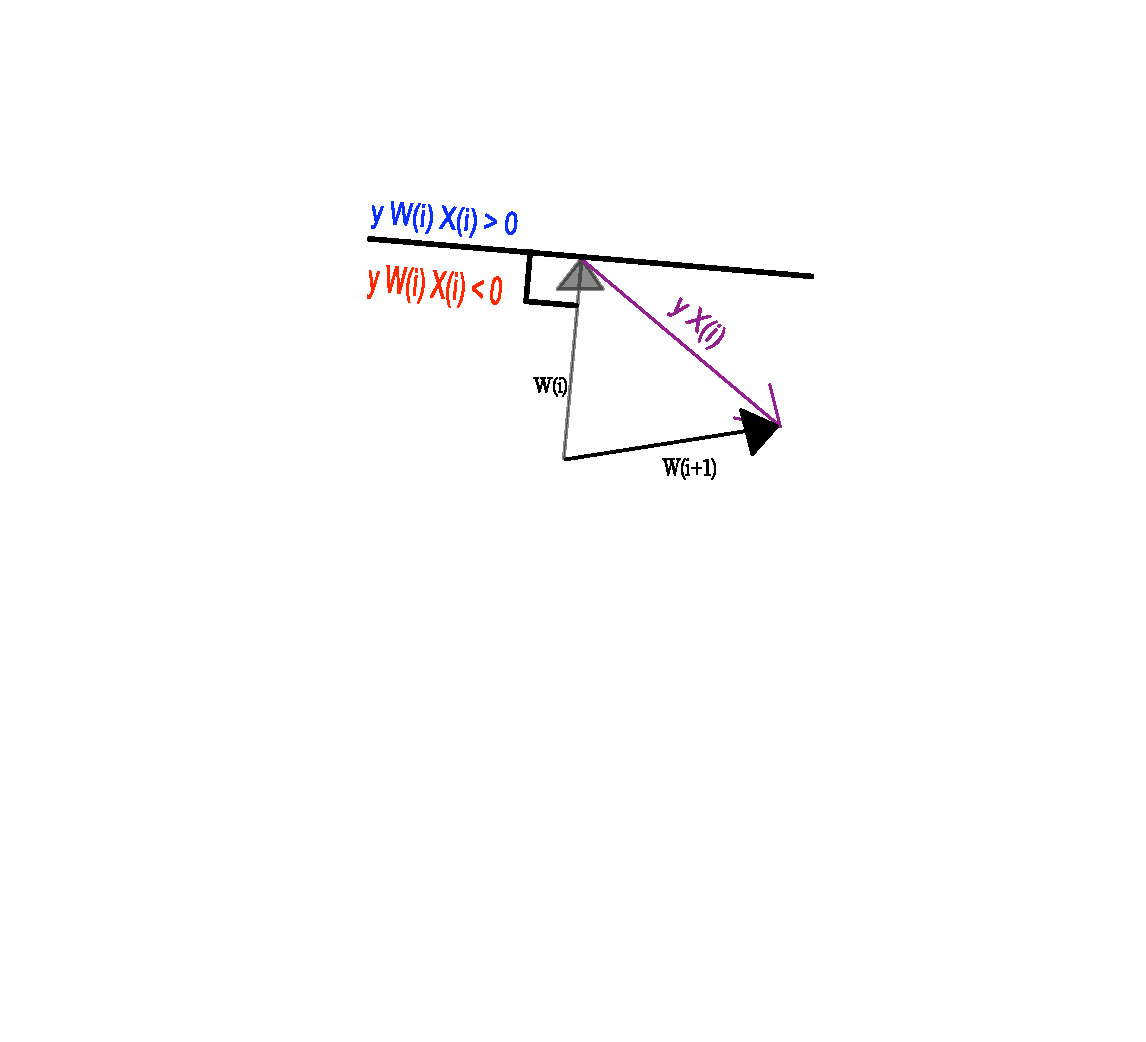
\includegraphics[height=10cm]{PerceptronAnim/PerceptronError.pdf}
\end{frame}

\begin{frame}
\frametitle{Upper bound on $\| \W_i \|$}
\pause
Proof by induction
\begin{itemize}
\item Claim: $ \| \W_{i} \|^2 \leq i R^2 $
\item Base: $i=0$, $\|\W_0\|^2 = 0$
\item Induction step (assume for $i$ and prove for $i+1$):\\
$ \| \W_{i+1} \|^2 \leq \|\W_i\|^2 + \|\X_i\|^2 $ \\
$\leq \|\W_i\|^2 + R^2 \leq (i+1) R^2$

\end{itemize}
\end{frame}

\begin{frame}
\frametitle{Lower bound on $\| \W_i \|$}
\pause
$\|\W_i\| \geq \W_{i} \cdot \V$ because $\| \V \|=1$.\\
\pause
We prove a lower bound on $\W_{i} \cdot \V$ using induction over $i$
\begin{itemize}
\item Claim: $ \W_{i} \cdot \V \geq i g $
\item Base: $i=0$, $\W_0 \cdot \V = 0$
\item Induction step (assume for $i$ and prove for $i+1$):\\
$ \W_{i+1} \cdot \V  = \left( \W_i + \X_i y_i \right) \V$
\pause
$= \W_i \cdot \V + y_i \X_i \cdot \V$ \\
$\geq i g + g = (i+1) g$
\end{itemize}
\end{frame}

\begin{frame}
\frametitle{Combining the upper and lower bounds}
~\\
~\\
\pause
$$(ig)^2 \leq \|\W_i\|^2 \leq i R^2$$
\pause
Thus:
$$ i \leq \left(\frac{R}{g} \right)^2 $$
\end{frame}

%\iffalse %%%%%%%%%%%%%%%%%%%%%%%%%%%%%%%%%%%%%%%%%%%%%%%%%%%%%%%%%%%%%%%%%%
\section{Laplace law of succession}

\begin{frame}
\frametitle{Estimating the bias of a coin}

\begin{itemize}
\item We observe $n$ coin flips:\\
{\bf H,T,T,H,H,T,H,T,T}
\item
We want to estimate the {\bf probability} that the next flip will be {\bf H}ead.
\item
Natural Answer:
\[
\frac{\#\mbox{\bf H}}{n} = \frac{4}{9}
\]
\end{itemize}
\end{frame}

\begin{frame}
\frametitle{What if the estimation has to be done online?}

\begin{itemize}
\item We observe a {bf sequence} of coin flips, and have to predict the probability of {\bf H}ead at each step:
\\ $p_0$,\pause 
{\bf H},\pause 
$p_1$,\pause
{\bf T},\pause
$p_2$,\pause 
$\ldots$
\item
What would be a good value for $p_0$?
\item
For $p_1$?
\item
Laplace Law of succession
\[
\frac{\#\mbox{\bf H} +1}{n+2}
\]
\item 
Turns out that a better rule is 
\[
\frac{\#\mbox{\bf H} +1/2}{n+1}
\]
Krichevsky and Trofimov, 1981
\item
Why? 
\item 
What does ``better'' mean?
\end{itemize}
\end{frame}

\begin{frame}
\frametitle{Next time}
Analysis of the Hedge Algorithm.
\begin{itemize}
\item slides in \B{talk1.handout.pdf} on: \B{\tt
    https://github.com/yoavfreund/2020-Online-Learning}
\item {\bf Grading:} 4HW (40\%), Midterm (20\%) Final (40\%)
\item See you on Thursday!
\end{itemize}
\end{frame}
%\fi %%%%%%%%%%%%%%%%%%%%%%%%%%%%%%%%%%%%%%%%%%%%%%%%%%%%%%%%%%%%%%%%%%%

\end{document}


